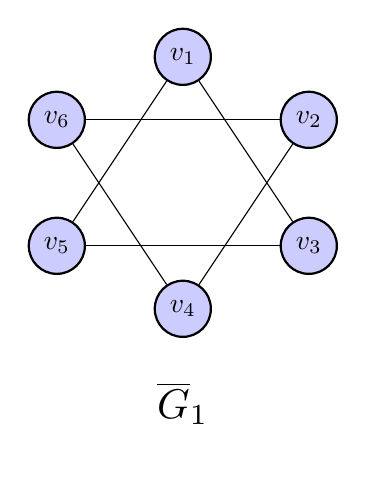
\begin{tikzpicture}
  [scale=.8,auto=left,every node/.style={circle,fill=blue!20,draw=black,thick}]
  \node (n1) at (2,4) {$v_1$};
  \node (n2) at (4,3) {$v_2$};
  \node (n3) at (4,1) {$v_3$};
  \node (n4) at (2,0) {$v_4$};
  \node (n5) at (0,1) {$v_5$};
  \node (n6) at (0,3) {$v_6$};

  % Aristas del complemento \overline{G}_1
  % Aristas rectas
  \draw (n1) -- (n3);
  \draw (n1) -- (n5);
  \draw (n2) -- (n4);
  \draw (n2) -- (n6);
  \draw (n3) -- (n5);
  \draw (n4) -- (n6);

  % Etiqueta \overline{G}_1 debajo del grafo
  \node[draw=none, fill=none, scale=1.5] at (2,-1.5) {$\overline{G}_1$};
\end{tikzpicture}
